% ============================================================
% image2 重绘（探三例1 · 正方体 ABCD-A_1B_1C_1D_1，E 在 A_1C_1 上）——TikZ 矢量片段
% 仅依赖 tikz。源自位图：工作区/字替对照-0909/variantF/media/media/image2.png（764×764px）
% 源排印宽 42.0mm ⇒ 1px = 42/764 = 0.054974 mm（本片段 x=1mm,y=1mm，坐标已按此折算）
% 线宽：源图实测 5.5~5.75px（竖/横各向异性）取 5.6px ⇒ 0.3080 mm ≈ 0.88 pt
% 虚线：源图实测 on 22px / off 15.5px ⇒ on 1.209mm off 0.852mm（周期 2.061mm）
% 点 E：源图实心圆 r=8.58px ⇒ r=0.472mm（直径 0.94mm），圆心落在 A_1C_1 上
% 标签：源自全品图=Times 系斜体变量＋直立下标；本片 $\mathit{X}_{\mathrm{1}}$（\mathit 走主字体斜体＝
%       Times New Roman Italic、\mathrm 走主字体直立数字，贴源图观感）；字号 14.53pt（源图大写 A 高
%       63px⇒3.425mm，已写入 every node 的 font=，宿主无需另设字号）。若宿主数学体本身即 Times 系
%       （unicode-math+Termes/XITS），可整体换回惯用的 $X_{1}$；下标比例差见核对表§偏差
% 注：题面 A_1E=¼A_1C_1，而源位图实测 E 落在 t=0.315（绘图不精确）；本片按位图复刻 t=0.315。
%       若须贴题面精确 ¼：把 \coordinate (E) 改为 ($(A1)!0.25!(C1)$)。
% 顶点（源图像素，子像素实测）：A(108.61,672.00) B(527.39,672.00) A1(108.61,253.00) B1(527.39,253.00)
%        C(683.00,514.86) C1(683.00,96.00) D(264.55,514.55) D1(264.55,96.00) E(289.54,203.58)
% 实线：AB BC CC1 C1B1 B1B BA1 A1A A1D1 D1C1 A1C1 ；虚线：AD DC DD1 AE
% ============================================================
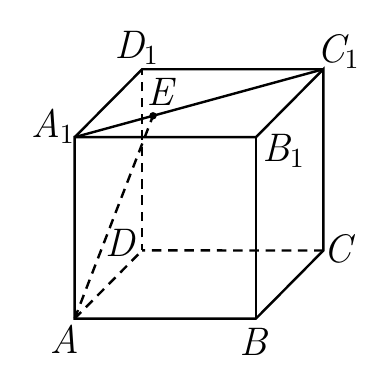
\begin{tikzpicture}[x=1mm,y=1mm,line width=0.308mm,line cap=butt,line join=miter,
                    every node/.style={font=\fontsize{14.53pt}{17.436pt}\selectfont}]
% ---- 坐标（mm，原点=位图左上角，y 向上） ----
\coordinate (A)  at (5.971,5.058);\coordinate (B)  at (28.993,5.058);
\coordinate (A1) at (5.971,28.092);\coordinate (B1) at (28.993,28.092);
\coordinate (C)  at (37.547,13.696);\coordinate (C1) at (37.547,36.723);
\coordinate (D)  at (14.543,13.713);\coordinate (D1) at (14.543,36.723);
\coordinate (E)  at (15.917,30.809);   % E = 线 A1C1 ∩ 线 AE（源图 t=0.315，见核对表）
% ---- 虚线（隐藏棱 AD、DC、DD1 与辅助线 AE）----
\def\qon{1.209mm}\def\qoff{0.852mm}
\draw[dash pattern=on \qon off \qoff, dash phase=0.033mm] (A)--(D);    % 首段墨迹距 A 36.9px
\draw[dash pattern=on \qon off \qoff, dash phase=0.825mm] (D)--(C);    % 自 D 起 22.5px 起墨
\draw[dash pattern=on \qon off \qoff, dash phase=0.399mm] (D)--(D1);   % 相位按 dash 中心拟合（自 D 起第1段中心 30.25px）
\draw[dash pattern=on \qon off \qoff, dash phase=0.049mm] (A)--(E);    % 首段墨迹距 A 36.6px
% ---- 实线：前面 ABB1A1、右面 BCC1B1、上面 A1B1C1D1、对角线 A1C1 ----
\draw (A)--(B)--(C)--(C1)--(B1)--(A1)--(A)--cycle;   % 外轮廓：A-B、B-C、C-C1、C1-B1、B1-A1、A1-A
\draw (B)--(B1);                                     % 前面右竖棱 B-B1
\draw (A1)--(D1)--(C1);                              % 上面后两条可见棱
\draw (A1)--(C1);                                    % 上面对角线（E 所在）
% ---- 点 E（实心圆）----
\fill (E) circle[radius=0.472mm];
% ---- 标签 ----
\node at (4.644,2.350) {$\mathit{A}$};
\node at (28.898,2.116) {$\mathit{B}$};
\node at (39.683,13.844) {$\mathit{C}$};
\node at (11.954,14.713) {$\mathit{D}$};
\node at (17.085,33.897) {$\mathit{E}$};
\node at (3.229,29.422) {$\mathit{A}_{\mathrm{1}}$};
\node at (32.520,26.320) {$\mathit{B}_{\mathrm{1}}$};
\node at (39.457,38.888) {$\mathit{C}_{\mathrm{1}}$};
\node at (13.870,39.477) {$\mathit{D}_{\mathrm{1}}$};
% ---- 外框＝源排印幅面 42x42mm（与源位图 764x764px 同幅；不含图形，只定画布大小，
%      比节点自然外框（44.7x43.5mm）更贴源幅面。集成方若要“紧框”，删掉这两行即可） ----
\pgfresetboundingbox
\path[use as bounding box] (0,0) rectangle (42,42);
\end{tikzpicture}
